%! TeX root = thesis.tex
\chapter{Discussion}\label{sec:discussion}
\IMRADlabel{discussion}
% \section{Discussion of Results}

% \section{Organizational Improvements}
% Despite the successes of the class 1 models, there is ample room for improvement.

% Despite long preparation, insufficent research was conducted examining the proposed methods, and whether or not they were suitable for this project.
% The issues regarding curvature and the selection of a height function could not have been foreseen during the research and planning phase of the project.
% However, the interaction of \textit{Interior Edge Extension} and curved edges could have been detected during the planning phase.

% \section{Curvature Selection}
% Curvature calculations: The curvature calculations seem to be correct.
It was discovered towards the end of the project that the \textit{height} function chosen as the input to Watershed segmentation, namely the magnitude of the gradient of curvature, did not work well for all edges as hoped.
Curvature, specifically Gaussian and RMS curvature, produces boundaries at ``hard'' model edges, but not at ``soft'' model edges.
If the bordering primitives are tangent or near tangent to one another the edge is considered soft; otherwise, it is considered hard.
The derivative of curvature however, is better suited to producing boundaries at soft edges, but produces ``double'' boundaries at hard edges.
Figures \ref{sfig:m7_rmsk} and \ref{sfig:m7_gradk} give a visual comparison of the singular and double edges produced at hard edges.
% On the other hand, the derivative of curvature (the "magnitude" thereof as used in this work) is more useful for soft edges, but produces a "double" edge at hard edges, which can lead to poor (watershed) segmentation results.
\begin{figure}[htb]
	\centering
	\begin{subfigure}[t]{0.42\textwidth}
		\centering
		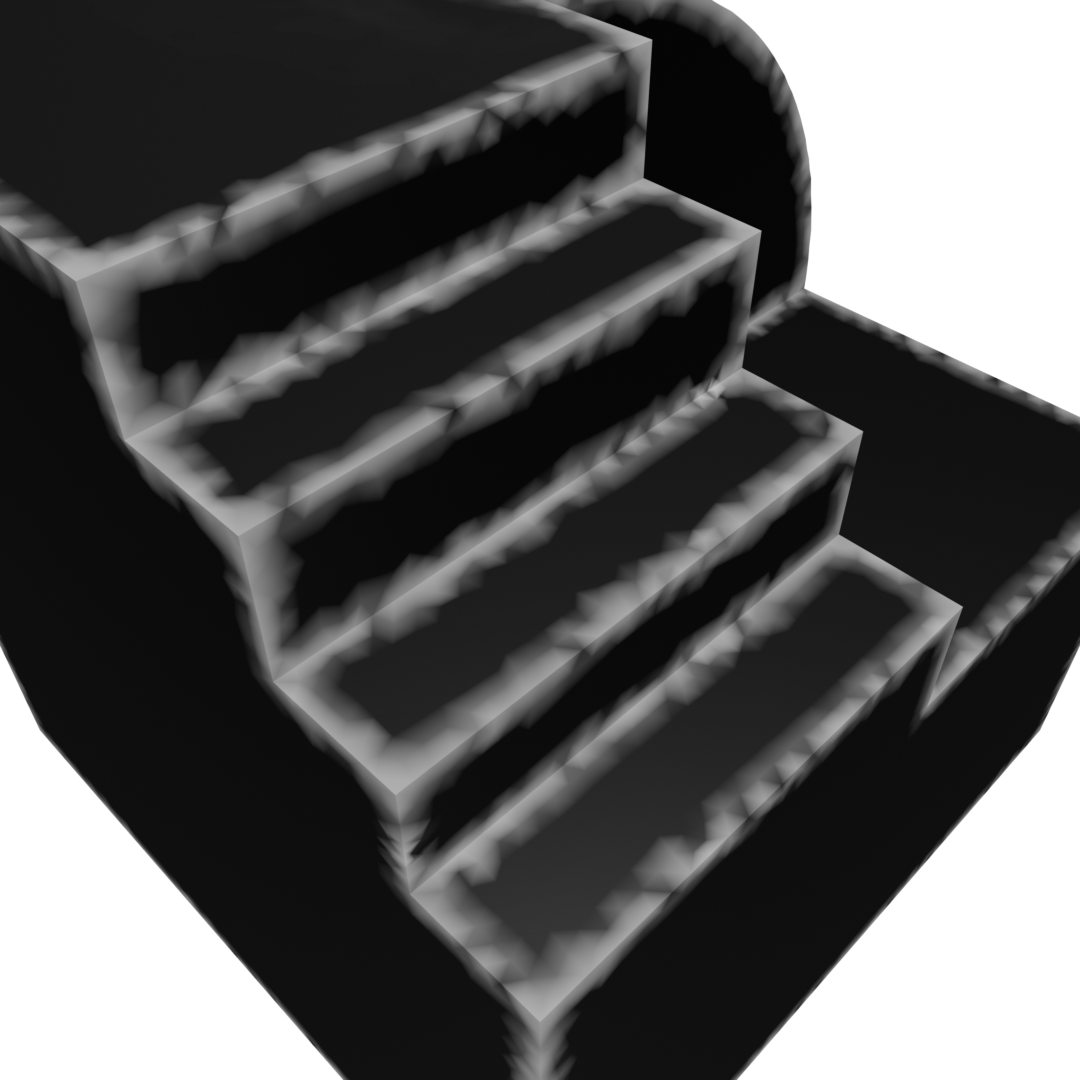
\includegraphics[width=\linewidth]{../resources/curvature/m7120369_rmsk.png}
		\caption{RMS curvature shown in grayscale.}
		\label{sfig:m7_rmsk}
	\end{subfigure}
	\hfill
	\begin{subfigure}[t]{0.42\textwidth}
		\centering
		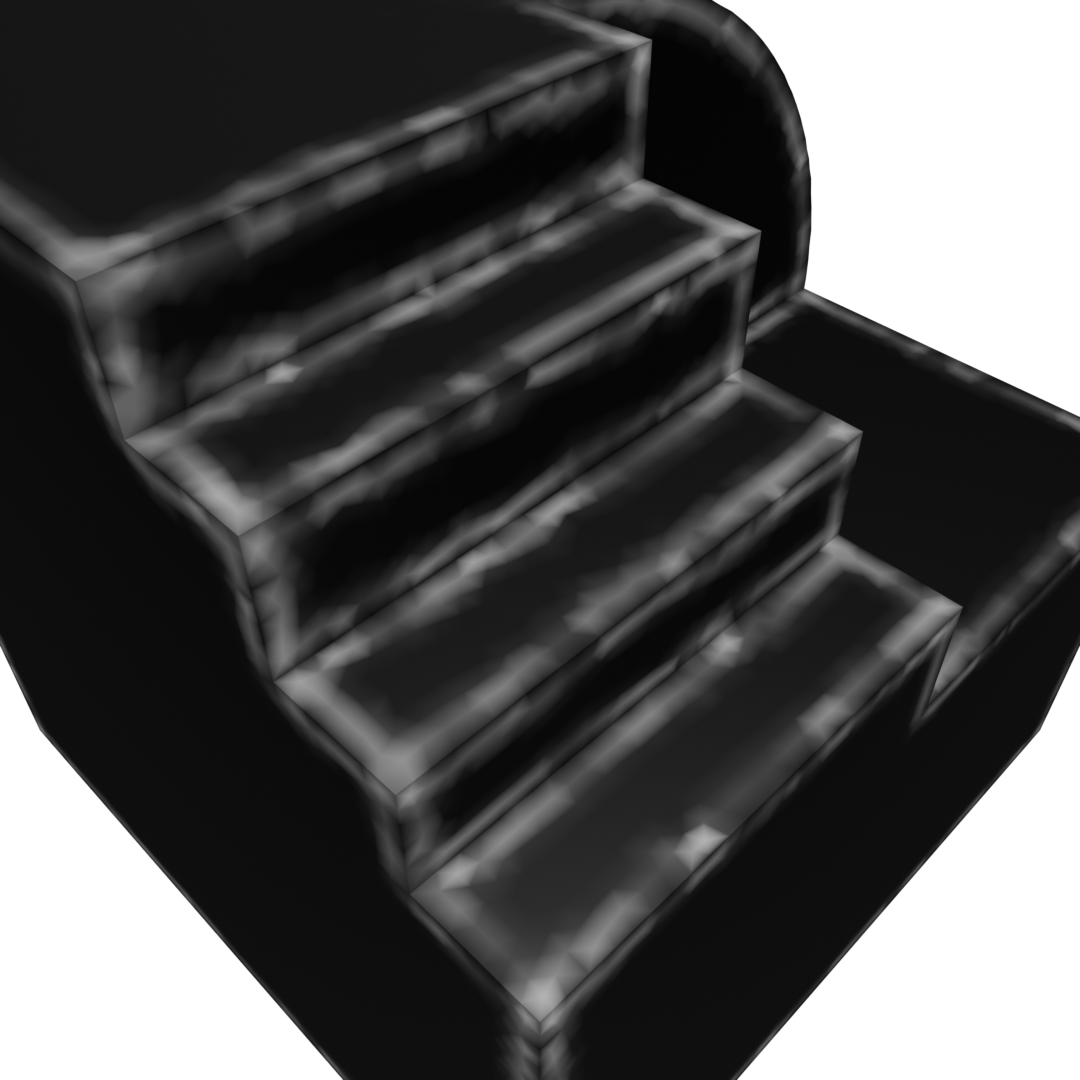
\includegraphics[width=\linewidth]{../resources/curvature/m7120369_gradk.png}
		\caption{Curvature gradient magnitude shown in grayscale.}
		\label{sfig:m7_gradk}
	\end{subfigure}
	\caption{Comparison of the RMS curvature and the curvature gradient magnitude height functions.}
\end{figure}

Intuitively, this is a problem because the resultant mesh regions should be divided at hard edges, rather than occupy them.
Recall that the first step of \textit{Watershed Segmentation} starts a mesh region at every local minima and minimum plateau.
This means that Watershed will create mesh regions directly on the hard edge due to the double edge produced when using the gradient magnitude as Watershed's height function.
Figures \ref{sfig:m7_rmsk_init} and \ref{sfig:m7_gradk_init} present the initial mesh regions created from the mesh heights shown in Figures \ref{sfig:m7_rmsk} and \ref{sfig:m7_gradk}, respectively.

\begin{figure}[htb]
	\begin{subfigure}[t]{0.42\textwidth}
		\centering
		
\includegraphics[width=\linewidth]{../resources/curvature/m7120369_rmsk_init.png}
		\caption{%
Initialized mesh regions with RMS curvature as the height function.
Black indicates unindexed vertices, while the other colors indicate a mesh region.
}
		\label{sfig:m7_rmsk_init}
	\end{subfigure}
	\hfill
	\begin{subfigure}[t]{0.42\textwidth}
		\centering
		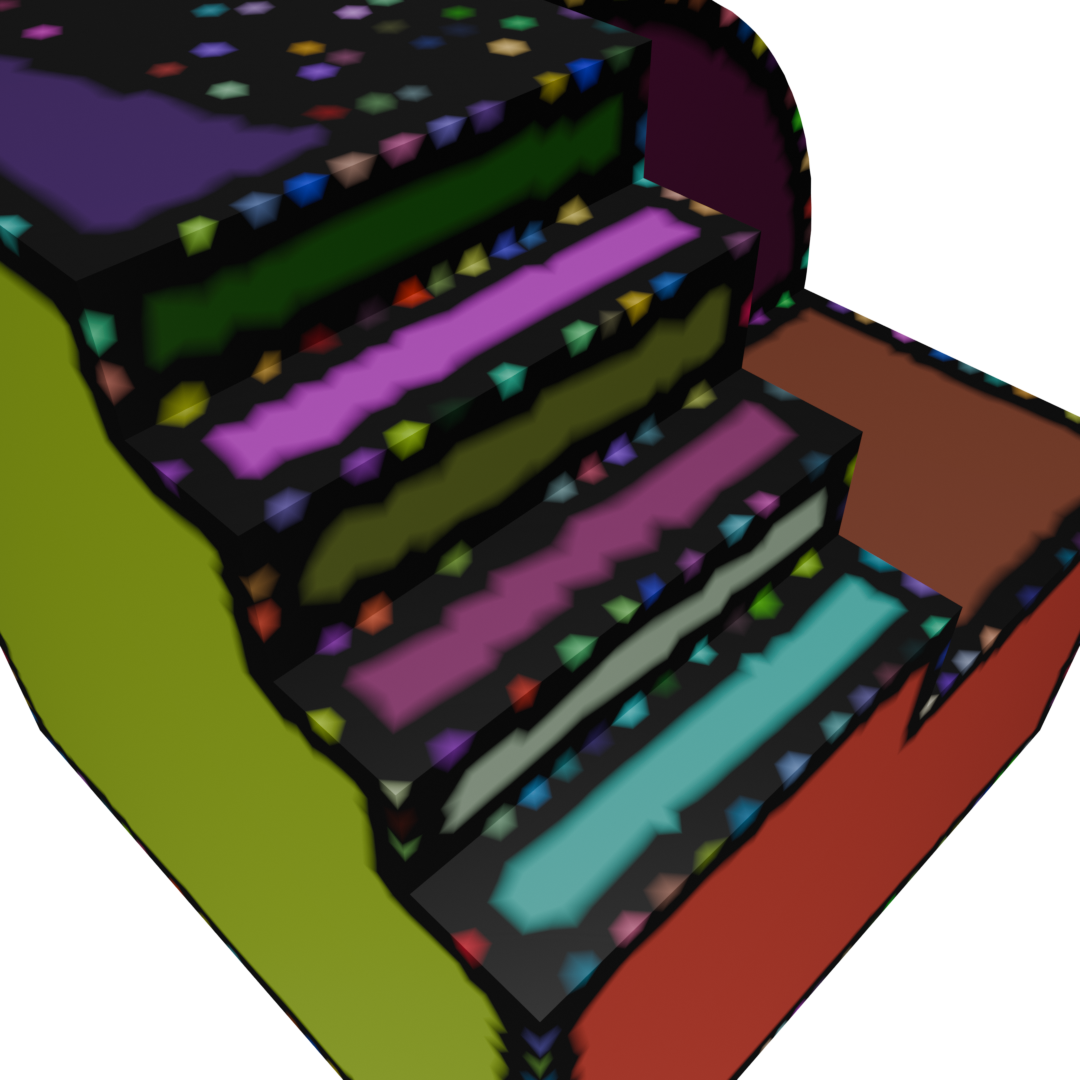
\includegraphics[width=\linewidth]{../resources/curvature/m7120369_gradk_init.png}
		\caption{%
Initialized mesh regions with curvature gradient magnitude as the height function.
Black indicates unindexed vertices, while the other colors indicate a mesh region.
}
		\label{sfig:m7_gradk_init}
	\end{subfigure}
	\caption{Comparison of Watershed's mesh region initialization from a mesh using RMS curvature as its height function (a) and a mesh using the curvature gradient magnitude as its height function (b).}
	% \label{fig:height_fn_comparison}
\end{figure}

% This can be seen in the initial mesh regions presented in Figures \ref{sfig:m7_rmsk_init} and \ref{sfig:m7_gradk_init}.
While the RMS curvature results \textit{do} show some local minima on hard edges, they are few and far between.
The gradient magnitude results show a myriad of local minima, and thus initialized mesh regions, on hard edges.
Because of \textit{Descent to Minima} these edge regions grow to encroach past the edge upon which they sit.
During \textit{Mini-Merge} these regions are merged into a larger neighboring region, forcing \textit{that} region to reach past its would-be edges.
The effect of this on the segmentation process is that during \textit{Surface Classification} the vertices from the ``spillover'' parts of the region were treated as outliers, resulting in those surfaces being classified as composite, rather than their true surface class.
% should be cleanly segmentable end up containing too much of adjacent surfaces to be classified as anything other than composite.
It was found through testing that this issue could be mitigated by increasing the density of the mesh.
Higher mesh density, especially at the true edges, limits the distance the edge regions may spread during \textit{Descent to Minima}.
Because the spillover vertices are closer to the edge, they are less likely to disqualify the region from being classified as its true surface class.
Because of this issue, the primary height function was reverted to RMS curvature.
This facilitated operating on models with hard edges, but made it[the algorithm] unsuitable for models with soft edges.

Two possible solutions to this were devised.
The first possible solution would be to create a height function that combines takes into account both curvature and its derivative.
Another idea is to alternate between using a curvature based height function and a curvature derivative based height function during \textit{2D Segmentation}.
The mesh would be segmented initially with RMS curvature as the height function, and during the next round of segmentation the curvature gradient magnitude would be used as the height function to handle any soft edges.

% \section{Watershed Segmentation}
Watershed segmentation, as implemented here, generally functioned as intended.
% Despite this, some models encountered issues during Watershed segmentation on well defined edges.
Although, after reverting the height function to RMS curvature, the second Watershed step, \textit{Minima Expansion}, caused regions to expand far further than they had when the height function was set to the curvature gradient.
Because the expansion exponent in \textit{Minima Expansion} is fixed throughout segmentation, an unsuitable value cannot be escaped or overcome the way a high merge exponent can be.
Thus \textit{Minima Expansion} was disabled.
% Based on the results observed, the cause of any segmentation issues is believed to lie with the height function chosen.
The other main modification to the Watershed process, namely the \textit{Mini-Merge} step, was found to qualitatively improve the Watershed process by reducing over-segmentation.
% Though not thoroughly tested, the Watershed modifications made in this work are expected to have been non-detrimental.
The \textit{Mini-Merge} step however, was found to occasionally cause over-merging on low-density meshes.
This was sometimes the case with narrow planar regions, but was generally resolved through adequate remeshing.
While remeshing of models to further development is acceptable, in order for the system to be properly automated, either a more reliable solution for handling narrow surface regions should be developed, or remeshing should be incorporated into the pipeline.
% , either of the entire model, or of the target feature.
% NOTE: hm, could word it less vaguely...

% \section{Surface Classification}
Of the implemented primitives, plane and elliptic cylinder, \textit{Surface Classification} works as intended.
Expanding this project to handle the third proposed primitive, ellipsoids, would be relatively straightforward, given that Eberly's work on ellipses extends to ellipsoids~\cite{GeoTools_pt_to_ellipse}.
Should the approach of primitive segmentation and classification be pursued further, the functionality to handle more primitives will be necessary.
Beyond ellipsoids, the main remaining geometric primitives are the cone and torus.
For both of these Eberly once again offers solutions~\cite{GeoTools_least_squares_fitting}, though fitting a cone to 3D points can likely be simplified by exploiting the input mesh's normals.
% The surface classification methods presented here, although they represent earnest attempts, are generally unreliable. -> less so since classifiers were replaced with pure regression.

% \section{Geometry Simplification}
% The region of geometric feature space where GS reliably produces simplified geometry, is smaller than hoped.
The range of geometric features and types of models from which \textit{Geometry Simplification} can reliably produce simplified geometry is smaller than hoped.
Readers may notice that plenty class 1 test shapes, the shapes for which paths were expected to be easily plannable, are marked as failures.
Two causes were identified: short edges and invalid corners.

Short edges, specifically narrow regions, were actually expected to be an issue during Watershed segmentation, but this was generally solved by increasing the mesh density and reverting the height function to RMS curvature.
Readers may recall that the purpose of the \verb|if| statement in Algorithm~\ref{alg:shared_edges_2} in \textit{Create Shared Edges} is to filter out tiny edges assumed to be mistakes.
Through testing this fake edge test showed false positives.
That is, legitimate edges were filtered out because they contained too few vertices.
% TODO: Perhaps add a picture of a model with narrow / short edges to illustrate the point?
This too can be resolved by locally increasing the mesh density to the point that edges formed have sufficient vertices to escape omission.
Though this again weakens the automation aspect of the project.
A better solution would be to develop an edge filter not based on the number of vertices contained in the given edge.
Possible implementations to this are still being pondered.

The second issue hampering successful path planning of class 1 models are ``invalid corners''.
When dealing with models that contain only planar surfaces, all corners will adjoin at least three surfaces.
During testing instances of corners that connected only two surfaces were encountered, which caused errors during the \textit{Extend Shared Edges} step.
These are the aforementioned invalid corners.
% The exact cause of these invalid corners is unknown, but corners where four or more edges converged tended to be segmented poo
% ... but corners where four or more edges converged tended to be segmented poo
The segmentation of the regions around corners where four or more edges converged tended to be qualitatively poorer than not.
The regions around corners where four or more edges converged were prone to qualitatively poorer segmentation results.
Though the exact cause of these invalid corners is unknown, it was observed that the regions of poorer segmentation tended to correlate with their occurence.
\iffalse
This issue can be illustrated with the help of the log file snippet shown in Listing \ref{lst:log_snippet} below.
\begin{lstlisting}[
	frame=tb,captionpos=b,
	caption={Abbreviated list of shared corners created from a model with quad+ corners.},
	label=lst:log_snippet]
Idx 	Corner end-pts	->		Corner position
 5 { 21[s], 16[s], 13[s],  6[s] } -> -0.2551  0.25653  0.72552
 9 { 15[e], 12[e], 11[s],  4[s] } -> 0.51161  0.00025  0.36407
12 { 21[s], 13[s] } -> -0.25649  0.25789  0.72361
15 { 15[e], 11[s] } ->  0.51136  0.00301  0.36372
\end{lstlisting}
Listing \ref{lst:log_snippet} lists some of the shared corners created from a model with quad+ corners.
The columns provide, in order, the shared corner's index, its edge tips, and its position.
The listing has been trimmed to only show those four shared corners for brevity.
Regarding the edge tips, the number indicates the edge's index and the \verb|s| and \verb|e| in the brackets correspond to the \verb|s|tart and \verb|e|nd tip of the edge.
Notice that corner 5 contains both of 12's edge tips, and that their positions are approximately coincident.
Thus, given corner 5, corner 12 is redundant.
Corners 9 and 15 have the same relationship, with corner 15 made redundant by corner 9.
These excess corners trip up (? maybe use more sophisticated word?) the program during execution of the \textit{Extend Shared Edges} step (see Section \ref{sec:extend_shared_edges}).
The quick solution to this issue is to filter out redundant and duplicate shared corners.
A better solution would be to determine how and why redundant shared corners were created at all.
This is a clear point of potential improvement, should this project be continued in the future.
\fi
% This is a minor issue that could be solved by filtering out the redundant or duplicate shared corners, and would have been solved given more development time.
% Creating idealized forms from the mesh regions in \textit{Geometry Simplification} worked ok, but was not without issue.

Due to time constraints handling of cylindric regions was not fully implemented in the \textit{Geometry Simplification} step, and as such, future work should aim to rectify this.

% \section{2D Segmentation}
% NOTE: ensure that this line stays with the enumerate below it
The stated goals of the \textit{Interior Edge Extension}\cite{IntEdgeExt} are:
\begin{enumerate}
	\item to minimize the number of changes in direction of the planned paths.
		This goal leads to the optimization requirement of minimizing the sum of cell widths when solving the weighted set coverage problem.
	\item to produce convex cells.
\end{enumerate}

Minimizing the number of direction changes is of value if the cost in time or energy of a direction change is non-negligible, as is the case for mobile robots such as automated agriculture machines, AUVs, and to a lesser degree UAVs.
However the cost of direction change for a robot arm is minimal.
% Furthermore, the envisioned end-effector tool is equally effective in its surface treatment moving in the positive or negative direction normal to the laser plane.
Furthermore, the envisioned end-effector tool is a planar ablation laser, which has no forward or backward direction, only the direction normal to the laser plane.
% (? rethink previous sentence...?)
That is, while a Roomba would be less effective if it were to traverse its environment backwards, the laser module suffers no such loss of efficacy.
% a ``planar laser'' (? revisit with better wording)
% need not rotate at each switchback because it is
Hence, the goal of minimzing the number of switchbacks was unnecessary for this work.

Nielsen et al.\ do not explain why the final polygons should be convex, treating it as a given.
Boustrophedon path planning requires cells to be \textit{semi}-convex, not necessarily truly convex.
This is illustrated in Figure \ref{fig:bpath_semi_convex} below.

\begin{figure}[htb]
	\centering
	\begin{tikzpicture}[scale=1.0]
		\begin{axis}[
			axis lines=none,
			scale mode=scale uniformly,
			enlargelimits=false,
		]
		\addplot
			table[mark=none,col sep=comma] {../resources/boustrophedon/ex_2_polygon.csv};
		\addplot
			table[mark=none,col sep=comma] {../resources/boustrophedon/ex_2_path.csv};
		\end{axis}
	\end{tikzpicture}
	\caption{Boustrophedon path planning successfully performed on a semi-convex shape}
	\label{fig:bpath_semi_convex}
\end{figure}

For semi-convex polygons the best sweep direction may no longer coincide with the polygon's longest edge, and thus cannot be chosen based on that.
The sweep direction must be chosen such that a line parallel to the sweep direction reaches the entire polygon when swept along the shift direction.
% A formal definition of ``semi-convex'' is beyond the scope of this work, and left for future work, but ..?
Although a formal definition of ``semi-convex'' is beyond the scope of this work, an informal one may be attempted.

% \subsection{Isovist Line}
% TODO: new name... "bivist line" ?
To define a useful measure of "semi-convexity" the notion of the isovist is helpful.
Benedikt gives the definition of an isovist as "the set of all points visible from a given vantage point in space and with respect to an environment"\cite{Isovists}.
While the isovist concept is primarily used in architecture and urban spaces, it can also be applied to computational geometry.
In the \textit{art gallery problem} each guard represents an isovist, and the solution to a given art gallery problem is the minimum number of isovists to completely cover the given environment.
A similar problem in computational geometry is the \textit{watchman route problem}, in which the a single mobile watchman is tasked with guarding an environment with obstacles.
The challenge lies in determining the shortest path the watchman should take to observe the entire environment.
Determining a polygon's ``semi-convexity'' draws on both of these problems by reducing the number of guards is to one, whose scope of observation is further reduced to a single line in both directions, but who \textit{is} allowed to move perpendicular to the viewing direction.
% Extending the art gallery problem to create a semi-convexity-test for a polygon, the number of guards is reduced to one, whose scope of observation is further reduced to a single line in both directions, but who \texti{is} allowed to move perpendicular to the viewing direction.
If ``guarding'' the polygon this way is feasible, then the polygon is at least semi-convex, and boustrophedon path planning may be applied, with the shift direction set to the guard's direction of movement, and the sweep direction perpendicular thereto.
Naturally, convex polygons pass this test as well.
% Each guard is reduced to looking along a single line in both directions, but is allowed to move along a line perpendicular to the viewing direction.

Another issue with \textit{Interior Edge Extension} is how it handles round edges.
A smooth round edge, such as the one shown in Figure \ref{sfig:interior_curve}, theoretically has an infinite number of infinitesimal edges.
Performing \textit{Interior Edge Extension} on such a shape would naturally be impossible.
\begin{figure}[htb]
	\centering
	\begin{subfigure}[t]{0.3\textwidth}
		\centering
		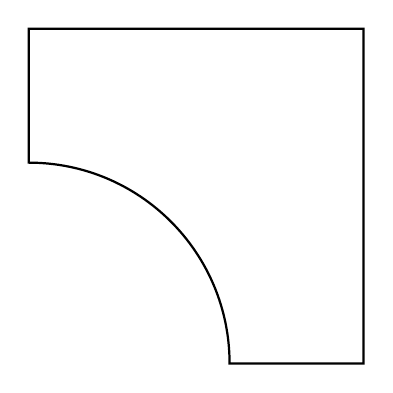
\begin{tikzpicture}[scale=0.85]
\draw[thick] (0,3) arc[start angle=90, delta angle=-90, radius=3] -- (5,0) -- (5,5) -- (0,5) -- cycle;
		\end{tikzpicture}
		\caption{Concave shape with an interior curve.}
		\label{sfig:interior_curve}
	\end{subfigure}
	\hfill
	\begin{subfigure}[t]{0.3\textwidth}
		\centering
		\begin{tikzpicture}[scale=0.85]
\clip (0,0) rectangle (5,5);
\draw[thick] (0,3) arc[start angle=90, delta angle=-90, radius=3] -- (5,0) -- (5,5) -- (0,5) -- cycle;
\foreach \a in {15,30,...,75} {
	\draw[red, dashed] ($(\a:3)+(\a-90:5)$) -- +(\a+90:10);
}
		\end{tikzpicture}
		\caption{%
The curve's line segments are extended.
% The curve has been discretized into 6 equal length segments.
% The dashed red lines show the result of extending the interior edges.
}
		\label{sfig:int_curve_ext}
	\end{subfigure}
	\hfill
	\begin{subfigure}[t]{0.3\textwidth}
		\centering
		\begin{tikzpicture}[scale=0.85]
\begin{axis}[
	anchor=origin,
	width=5.8cm,
	scale only axis,
	axis lines=none,
	scale mode=scale uniformly,
	enlargelimits=false,
]
\addplot[thick]
	table[mark=none,col sep=comma] {../resources/boustrophedon/ex_3_polygon.csv};
\addplot
	table[mark=none,col sep=comma] {../resources/boustrophedon/ex_3_path.csv};
\end{axis}
		\end{tikzpicture}
	\end{subfigure}
	\caption{%
Subfigure (a) gives an example shape that \textit{Interior Edge Extension} is not able to handle well.
In Subfigure (b) the shape's curved edge has been discretized into 6 segments.
Assuming a discretization of the curve into 6 equal segments, Subfigure (b) shows the extended edges of that curve as dashed red lines.
The boustrophedon path shown in Subfigure (c) illustrates that it is not even neecessary for the example shape to be segmented.
}
\end{figure}
Curves encountered by \textit{Geometry Simplification} are stored as discretized approximations.
Curves on a 3D mesh are inherently discrete and the number of their edge segments is finite.
Despite this, \textit{Interior Edge Extension} is still ill-suited to handling curves.
Suppose the curved edge shown in Figure \ref{sfig:interior_curve} were discretized into 6 equal line segments.
Figure \ref{sfig:int_curve_ext} shows the resultant extended interior edges from such a discretization.
Even with the best computational resources, most of the ``optimal'' sub-regions produced would likely be long slip triangles.
\textit{Interior Edge Extension} is only useful for simple polygons with all straight edges.
% Technically, having a curved edge would disqualify a shape from _being_ a "polygon"

% \section{Cellular Path Planning}
Cellular path planning using boustrophedon path planning worked as expected.
There was potential for expansion, such as allowing the TSP to potentially determine the path start point on the polygon.
This is left for a future expansion of the project, in which the TSP is fully implemented.

% \section{Traveling Salesman Problem}
Although part of the original plan, the TSP was not implemented in this work.
A natural extension of this project would be to implement a TSP function to join the individually planned surface paths.

